%% 11/23/2015
%%%%%%%%%%%%%%%%%%%%%%%%%%%%%%%%%%%%%%%%%%%%%%%%%%%%%%%%%%%%%%%%%%%%%%%%%%%%
% AGUJournalTemplate.tex: this template file is for articles formatted with LaTeX
%
% This file includes commands and instructions
% given in the order necessary to produce a final output that will
% satisfy AGU requirements.
%
% You may copy this file and give it your
% article name, and enter your text.
%
%%%%%%%%%%%%%%%%%%%%%%%%%%%%%%%%%%%%%%%%%%%%%%%%%%%%%%%%%%%%%%%%%%%%%%%%%%%%
% PLEASE DO NOT USE YOUR OWN MACROS
% DO NOT USE \newcommand, \renewcommand, or \def, etc.
%
% FOR FIGURES, DO NOT USE \psfrag or \subfigure.
% DO NOT USE \psfrag or \subfigure commands.
%%%%%%%%%%%%%%%%%%%%%%%%%%%%%%%%%%%%%%%%%%%%%%%%%%%%%%%%%%%%%%%%%%%%%%%%%%%%
%
% Step 1: Set the \documentclass
%
% There are two options for article format:
%
% 1) PLEASE USE THE DRAFT OPTION TO SUBMIT YOUR PAPERS.
% The draft option produces double spaced output.
%
% 2) numberline will give you line numbers.

%% To submit your paper:
\documentclass[draft,linenumbers]{agujournal}
%\draftfalse

%% For final version.
% \documentclass{agujournal}

% Now, type in the journal name: \journalname{<Journal Name>}

% ie, \journalname{Journal of Geophysical Research}
%% Choose from this list of Journals:
%
% JGR-Atmospheres
% JGR-Biogeosciences
% JGR-Earth Surface
% JGR-Oceans
% JGR-Planets
% JGR-Solid Earth
% JGR-Space Physics
% Global Biochemical Cycles
% Geophysical Research Letters
% Paleoceanography
% Radio Science
% Reviews of Geophysics
% Tectonics
% Space Weather
% Water Resource Research
% Geochemistry, Geophysics, Geosystems
% Journal of Advances in Modeling Earth Systems (JAMES)
% Earth's Future
% Earth and Space Science
%
%

\journalname{JGR-Planets}


\begin{document}

%% ------------------------------------------------------------------------ %%
%  Title
%
% (A title should be specific, informative, and brief. Use
% abbreviations only if they are defined in the abstract. Titles that
% start with general keywords then specific terms are optimized in
% searches)
%
%% ------------------------------------------------------------------------ %%

% Example: \title{This is a test title}

\title{Multi-view shape-from-shading for Mars}

%% ------------------------------------------------------------------------ %%
%
%  AUTHORS AND AFFILIATIONS
%
%% ------------------------------------------------------------------------ %%

% Authors are individuals who have significantly contributed to the
% research and preparation of the article. Group authors are allowed, if
% each author in the group is separately identified in an appendix.)

% List authors by first name or initial followed by last name and
% separated by commas. Use \affil{} to number affiliations, and
% \thanks{} for author notes.
% Additional author notes should be indicated with \thanks{} (for
% example, for current addresses).

% Example: \authors{A. B. Author\affil{1}\thanks{Current address, Antarctica}, B. C. Author\affil{2,3}, and D. E.
% Author\affil{3,4}\thanks{Also funded by Monsanto.}}

\authors{Oleg Alexandrov\affil{1} and Ross A. Beyer\affil{2,1}}

\affiliation{1}{NASA Ames Research Center}
\affiliation{2}{Sagan Center at the SETI Institute}
%(repeat as many times as is necessary)

%% Corresponding Author:
% Corresponding author mailing address and e-mail address:

% (include name and email addresses of the corresponding author.  More
% than one corresponding author is allowed in this LaTeX file and for
% publication; but only one corresponding author is allowed in our
% editorial system.)

% Example: \correspondingauthor{First and Last Name}{email@address.edu}

\correspondingauthor{Ross Beyer}{rbeyer@seti.org}

%% Keypoints, final entry on title page.

% Example:
% \begin{keypoints}
% \item	List up to three key points (at least one is required)
% \item	Key Points summarize the main points and conclusions of the article
% \item	Each must be 100 characters or less with no special characters or punctuation
% \end{keypoints}

%  List up to three key points (at least one is required)
%  Key Points summarize the main points and conclusions of the article
%  Each must be 100 characters or less with no special characters or punctuation

%\begin{keypoints}
%\item empty
%\end{keypoints}

%% ------------------------------------------------------------------------ %%
%
%  ABSTRACT
%
% A good abstract will begin with a short description of the problem
% being addressed, briefly describe the new data or analyses, then
% briefly states the main conclusion(s) and how they are supported and
% uncertainties.
%% ------------------------------------------------------------------------ %%

%% \begin{abstract} starts the second page

\begin{abstract}
This work presents a practical, usable Shape-from-Shading algorithm that works for Mars.
We model the haze in the Mars atmosphere, and find a best fit reflectance model using low
resolution CTX images and a high-resolution CTX DEM, that we use to enhance this DEM, 
which we compare to an even higher resolution HiRISE DEM.
\end{abstract}


%% ------------------------------------------------------------------------ %%
%
%  TEXT
%
%% ------------------------------------------------------------------------ %%

%%% Suggested section heads:
% \section{Introduction}
%
% The main text should start with an introduction. Except for short
% manuscripts (such as comments and replies), the text should be divided
% into sections, each with its own heading.

% Headings should be sentence fragments and do not begin with a
% lowercase letter or number. Examples of good headings are:

% \section{Materials and Methods}
% Here is text on Materials and Methods.
%
% \subsection{A descriptive heading about methods}
% More about Methods.
%
% \section{Data} (Or section title might be a descriptive heading about data)
%
% \section{Results} (Or section title might be a descriptive heading about the
% results)
%
% \section{Conclusions}

\section{Introduction}

Shape-from-Shading (SfS), also known as photoclinometry, is a set of
techniques for recovering surface relief based on variation in light
intensity recorded in images. 

In our paper \cite{alexandrovmulti}, we described a Shape-from-Shading implementation
and its application in creation of high-resolution Lunar Digital Elevation Models (DEMs) based on LRO NAC
images. Here we extend and validate that approach for Mars imagery. 

We proceed in a manner broadly similar to \citep{wohlfarth2018high}, in that we model the haze on Mars as an additive contribution to the image formation model, and we use that to obtain enhanced terrain models. Just as them, we employ CTX images to create a terrain model with SfS, and use a pre-existing HiRISE DEM for validation. We take advantage of the fact that the Mars Reconnaissance Orbiter (MRO) mission has two cameras: CTX, which acquires images at 6 meters per pixel, and HiRISE, whose images are at 0.25 m pixel, and the fact that there exist pre-existing DEMs made with state-of-the-art software from HiRISE images, which can be used to validate any DEMs created with SfS from the lower-resolution CTX images.   

There are several differences in our approach which make it more realistic. First, we model not only the haze, but also find a best fit reflectance model, which increases the accuracy. Second, to infer the haze coefficients they make use of the same high-resolution HiRISE DEM which they later use for validation. Once they learned the haze coefficients, they blur the HiRISE DEM, run SfS on it, and get a result closer to that high-resolution DEM than what they start with. 

We do not use the same HiRISE DEM for both training and validation, which can influence the results. We work with CTX images from the beginning to the end, and we use the HiRISE DEM for validation only. We achieve this by creating a high-resolution CTX DEM (which is much lower resolution than HiRISE), then use this one together with lower-resolution CTX images (whose resolution is comparable to the effective resolution of this DEM) to infer the haze and exposure values. Then we use these on the original CTX images to enhance the high-resolution CTX DEM which we then compare with the HiRISE DEM.  

Another difference is that when we find the best exposure and haze coefficients, we also determine the best-fitting reflectance model. Lastly, we use multiple CTX images (two and up to four), rather than just one. 

Our SfS implementation is not only an algorithm or some research code but released as a software program, called \texttt{sfs}, as part
of the NASA Ames Stereo Pipeline (ASP) \citep{ASP2017}, a collection of
open-source software for stereogrammetry and geodesy, available
under the Apache~2.0 license at: \\

\begin{center}
https://github.com/NeoGeographyToolkit/StereoPipeline
\end{center}

The program works with camera models provided by the Integrated
Software for Imagers and Spectrometers, version 3 \citep[ISIS3,][]{2017LPI....48.2739S,ISIS_website},
which is the standard for NASA planetary missions and other camera models for Earth observing satellites that ASP supports. The \texttt{sfs} tool has detailed documentation
and usage examples, with pre-compiled binaries for Linux and macOS.

\section{The Algorithm}

\subsection{The Cost Function}

We represent the terrain as a function $h(x,y)$, describing the
heights.  The coordinates $(x,y)$ are locations in a projection on planet's surface. Any projection can be selected, but it is advantageous to use the stereographic projection with the center of
projection at the center of the scene because it provides conformality, minimizes departures from the nominal scale, and avoids singularities at the poles and the 180$^{\circ}$ meridian.  We therefore use this projection in all of our examples.  Results can easily be resampled to other projections as desired.
This is sufficient for planetary applications,
though not for irregular shapes like asteroids. 

We assume that we
have one or more views of this terrain from satellite images, for
which we also know the position of the illumination source (the
Sun, which we represent as a point), as well as the positions and
orientations of the cameras. 

We set up a minimization problem whose optimal solution will be the desired $h(x,y).$
Following \citet{horn1990height}, we also consider as part of the optimization
the gradients (partial derivatives) $p(x,y)$ and $q(x, y)$ of $h(x, y)$,
that are varied independently, while having them connected to 
$h(x, y)$ via the integrability constraint as described below. This results in a less blurred 
solution if we instead expressed in the cost function these gradients as 
centered difference approximations of $h(x, y)$ without having them vary on their own. 

The cost function to be minimized is

\begin{eqnarray}\label{cost}
\int\!\! \int \! \sum_k \left[ I_k(h(x, y)) - T_k 
R_k(h(x, y), p(x, y), q(x,y)) - H_k \right]^2\, \nonumber \\             
+ \mu^2 \left\|\nabla^2 h(x, y) \right\|^2  \nonumber \\
+ \nu^2  
\left[ 
\left( \frac{\partial h}{\partial x}(x, y) - p(x, y)\right)^2  
+
\left( \frac{\partial h}{\partial y}(x, y) - q(x, y)\right)^2  
 \right] \nonumber \\
 + \lambda^2  \left[ h(x, y) - h_0(x, y) \right]^2
\, dx\, dy.
\end{eqnarray}
It is made of four terms, with weights $\mu > 0,$ $\nu>0,$ and $\lambda > 0$
attached to the last three. Here, $I_k(h(x, y))$ is the $k$-th camera image interpolated at
pixels obtained by projecting into the camera 3D points from the terrain
$h(x, y)$, $R_k(h(x, y), p(x, y), q(x,y))$ is the reflectance computed from the terrain for $k$-th image (section \ref{reflectance}), and $\left\|\nabla^2 h(x, y) \right\|^2 $ is the sum
of squares of all second-order partial derivatives of $h(x, y)$.

The first term is the brightness constraint. It enforces that the
simulated light intensity for the given terrain agrees well with
the light intensity as acquired by the camera. We assume that
image intensity is a first degree polynomial of the terrain reflectance,
with the coefficients $T_k$ and $H_k$ which we use to model the image exposure and
the atmospheric haze. Hence, we assume that haze can be modeled as simply an additive constant. 
This is following the "low-order polynomial" used in \citep{wohlfarth2018high}. 

It is the addition of $H_k$ which makes the model most different than what is used for the Moon,
which lacks atmosphere. And unlike for the Moon, here we do not model the albedo, 
as the CTX images, at least in the areas we examined, do not show any obvious albedo variation. 

In principle, the brightness constraint term should be sufficient. However,
\citet{horn1990height} indicates that in this case the algorithm
tends to be unstable and gets stuck in local minima, especially if
starting far from the solution. Hence the need for additional terms. 
The second term, weighed by $\mu > 0$, is usually called the smoothness constraint. It
enforces that the obtained terrain be reasonably smooth, and 
$\mu$ is used to control the smoothness amount. Its value should not be too large, as \citet{horn1990height}
also points out that if starting with the true solution, this term
will cause the optimization to move away from it, and it can also
over-smooth the result. However, one rarely gets to start with the
true solution, and in our experiments on real data, we 
found that it is necessary to use this term to get a good solution.

The third term, weighed by $\nu > 0,$ constrains $p(x, y)$ and $q(x,y)$ to not vary too much from
the true partial derivatives of the terrain $h(x, y).$ 
This is called the integrability constraint.

The SfS solution is known to reveal high resolution detail, yet it
may drift at larger spatial scales \citep{grumpe2014construction}.
That is the reason for the fourth term, weighted by $\lambda$, that
keeps the solution close to the initial guess terrain, $h_0(x, y)$. A
large value here is also undesirable, as it may constrain the
solution too much, hence some experimentation is usually necessary
to set this properly. The formulation of this term is not ideal, 
since penalizing departures from the a priori surface makes it harder to add local
details, which is the whole point of the process.  It would be better to penalize
the departure of the model only after smoothing $h(x, y)$ to an equivalent resolution from
the a priori terrain.  Given our implementation, doing it that way is impractical.  
While our approach is not the ideal formulation, we think that it achieves the same 
practical end, as long as care is taken to adjust the weight.

The variables of optimization are the terrain $h(x, y),$ the gradients 
$p(x, y)$ and $q(x, y)$ at each point
$(x, y)$, and the exposure, haze, and the reflectance model coefficients. 
All these can be independently fixed or varied. 

\subsection{The Reflectance Model}
\label{reflectance}

A key ingredient in the SfS problem is the reflectance model to be used, 
the quantity $R_k(h(x, y), p(x, y), q(x,y))$ (which we simply denote by $R$ below)
which describes
how a surface reflects light. The simplest model is the Lambertian,
\begin{equation}
R = \cos(i)
\end{equation}
which states that the reflectance at a terrain point is only dependent
on the incidence angle $i$ (the angle between the illumination
direction and the surface normal at a terrain point). This model is
often insufficient, and many adjustments to it have been used.

A reflectance model that is often used for the Moon is the lunar-Lambertian model
\citep{mcewen1996precise,lohse2006derivation}), which states that

\begin{equation}
R = \Lambda(\alpha) \frac{2\cos (i)}{\cos(i) + \cos(e)}
 + \left(1-\Lambda(\alpha)\right) \cos(i)
\end{equation}
where $e$ is the emission angle (the angle between the surface
normal to the terrain and the viewing direction), $\alpha$ is the phase
angle (the angle between the illumination and viewing directions), and
\begin{equation}
\Lambda(\alpha) = 1.0 + A\alpha + B\alpha^2 + C\alpha^3
\end{equation}
with
\begin{equation}
A = -0.019, \  B = 2.42\times 10^{-4}, \  C = -1.46 \times 10^{-6}.
\end{equation}
The particular parameterization for the behavior of $\Lambda(\alpha)$ can be highly
variable depending on photometric properties of the surface.  \citet{kirk2003photoclinometry}
describe the use of the ISIS3 program \texttt{pho\_emp\_local}, which is based on the ideas of \citet{mcewen1991photometric}, to
fit Minnaert or lunar-Lambertian models to a given Hapke model, and
may be useful for deriving parameters for $\Lambda(\alpha)$ in our
\texttt{sfs} program.

For Mars, one often employs the Hapke model \citet{hapke1993opposition}. We experimented with its formulation as given in \citep{fernando2013surface}. Both of these models have coefficients that need to be tuned. We optimized these coefficients as part of the SfS problem, as described later. 

It is important to note that $h(x, y)$ and the approximations $p(x, y)$ and $q(x,y)$ to its partial
derivatives are in a local projection for the given terrain. The sun position (which gives the 
illumination direction) and the camera position are all in a Cartesian coordinate system with its origin at the center of the planet (called the ECEF coordinates). Hence, one should compute the terrain points and surface normals in ECEF before proceeding with finding the angles $i, e, \alpha$ and the reflectance.  

\subsection{Handling Camera and Alignment Errors}
\label{bundleadjust}

The position and orientation of CTX images is quite imprecise. We use ASP's bundle adjustment program
to eliminate the camera errors before we create a DEM from the CTX images and refining it with SfS. To compare with the HiRISE DEM, we bring it into alignment to the CTX DEM using ASP's \texttt{pc\_align} tool which employs the Iterative Closest Point algorithm. 

If the illumination conditions for the images are very different, bundle adjustment may fail, as it becomes challenging to identify interest point matches across the images. We observed this for the Moon, but not for Mars, where the CTX (and HiRISE) images exhibit much less variation in illumination. To increase the likelihood of success of bundle adjustment, one can collect perhaps 5-10 images and order them so that the illumination condition difference between any consecutive images is not too large.   

The SfS tool can further refine the camera positions and orientations as part of the optimization, and this works very well, improving the quality of the results somewhat compared to keeping these quantities fixed. Yet we found that the preliminary bundle adjustment was sufficient on its own. 

\subsection{Discretization}

We discretize this problem using the finite difference method, hence the
domain of computation is a gridded rectangular box, and the quantities $h(x,y)$, $p(x,y)$, and $q(x, y)$
become matrices of numbers. Central differences are used to find
the partial derivatives.

The values of the these quantities at the boundary are kept fixed during optimization. The SfS tool allows these to be varied, yet better results were obtained if they are fixed instead.

\subsection{Initialization}

We assume that the cameras have been calibrated, and have known and accurate 
positions and orientations (handling camera errors was discussed in section \ref{bundleadjust}). 
A known position for the illumination point source is assumed as
well.

We typically use stereo on two of the images to get an initial guess
for the terrain $h(x, y)$ prior to running SfS, or we start with a
gridded LIDAR terrain (such as LOLA on the Moon). We also tested
our algorithm by initializing with a constant terrain. The results
returned by SfS in such a case look plausible but we did not quantify
their accuracy. In principle, an initial surface obtained by any
other means would also work.

%The initial albedo $A(x, y)$ is set to 1 everywhere (hence
%its scale is absorbed into the image exposure). Then, using the fact that
%the image intensity equals the image exposure times albedo times
%reflectance, we derive the initial camera exposure for image $k$ as:

\begin{equation}
T_k = \frac{ \int\!\! \int \! I_k(h(x, y)) \,dx\,dy }{ \int\!\! \int \! R_k(h(x, y)) \,dx\,dy}
\end{equation}
We set the initial haze values to be 0, and we initialize $p(x, y)$ and $q(x, y)$ as the partial derivatives of
$h(x, y)$. 

We found the weights $\mu, \nu,$ and $\lambda$ to be highly dependent 
on target surface properties and the resolved ground sample 
distance and (less so) on the illumination
conditions. Hence for each set up, several values of this parameter
should be tried (using a few or just one of the images for speed),
and its value can be chosen depending on which solution is closer
to the ground truth or otherwise results in a terrain of satisfactory
appearance, that is, a hillshaded image of this terrain appears
rather similar to the input images, without much noise or excessive
blur. 

The brightness term in the cost function is an image
intensity difference (squared), while the smoothness term is a
difference of elevations, measured in meters (then also squared).
It is perhaps not surprising that these cannot be easily reconciled,
hence for each target body and resolution a study needs to be done to evaluate the best value for this weight.

\subsection{Two-step Optimization}
\label{twostep}
The optimization problem, as set, has many variables, and likely many potential solutions. While in this paper we can always validate the result against the independently acquired high resolution HiRISE model,
the eventual goal may be to use SfS on HiRISE images themselves, when no other ground truth is available. 
Thus, it is desired to solve the problem in a way which may give some confidence in the results without
using an external ground truth. Hence, we employ an approach that is similar in spirit to \citep{wohlfarth2018high}, in first determining the exposure and haze for each image (and also refining the camera positions and reflectance coefficients), and later keeping them fixed when refining the terrain itself. 

We note that the exposure and haze are image-dependent, since each image is acquired independently, and the haze depends on the atmospheric conditions at the moment the image was taken as well as
the path through the atmosphere the rays traced from the ground to the camera. It is also expected
that the reflectance model depends on the surface geology of a particular terrain being model. 
Yet, these do not depend on the particular point on the terrain, pixel in the image,
or image resolution. Hence, given a particular set of CTX images, we train these quantities as follows.
We first run stereo with the full resolution CTX images, and create a terrain model. It is known that
the effective resolution of the terrain will be coarser than the image resolution. Therefore,  
we create this terrain model using a grid size that is 4 times the CTX image resolution, hence 
about 24 meters/pixel, at which it should be sufficiently accurate. We then resample the images by a factor of 4 as well, for consistency. We then minimize the cost function \ref{cost} using these resampled images while keeping the terrain fixed, and varying the image exposure, haze, model coefficients (and, if necessary, camera positions and orientations). Note that when doing this, all terms in that equation except the first are constant, hence the weights $\lambda, \mu, \nu$ are not important. 

We then use and keep fixed these learned quantities and the original full-resolution CTX images together with the terrain model obtained from this images, but this time the terrain is at the ground sample distance rather a multiple of 4 of it, to refine this terrain model using SfS, obtaining additional detail. We compare both the initial guess terrain and the final SfS result to the much higher resolution HiRISE DEM that is regridded to 6 m/pixel as well. 

\subsection{The Solver}

We use Google's CERES solver \citep{agarwal2012ceres} to minimize
the cost function. CERES is a highly versatile and very large-scale
least squares solver using the Levenberg-Marquardt algorithm. It
automatically computes partial derivatives numerically, creates a
sparse matrix for the problem which it inverts appropriately at
each iteration, and it handles properly situations when this matrix
is singular or not well-conditioned. All the user needs to do is
to provide routines for computing the terms in the cost function,
as well as stopping criteria. CERES is also able to prevent
unreasonably large cost function terms from dominating the computation,
though we did not use this feature.

\subsection{Selecting Input Images}

It is important when selecting images to choose ones with diverse illumination conditions, as then there is more information present, and it is easier to constrain the problem and get higher quality results. 

\section{Results}

\begin{table}[h]
\caption{Image parameters for SfS with CTX images}
\label{ctximages}
\centering
\begin{tabular}{lp{2cm}p{2cm}p{2cm}p{2cm}}
\hline
Product ID & Solar Longitude & Incidence Angle & Emission Angle & Sub Solar Azimuth \\
\hline
 F21\_044060\_1919\_XN\_11N045W  &   84.09  & 44.9  & 3.26   & 210.89 \\ 
 J04\_046526\_1918\_XN\_11N045W  &  177.28  & 51.71 & 3.92   & 178.94 \\ 
 F05\_037717\_1927\_XN\_12N045W  &  177.63  & 56.53 & 2.3    & 179.69 \\
 F10\_039735\_1919\_XN\_11N045W  &  273.99  & 55.37 & 0.31   & 144.28 \\ 
 F12\_040658\_1919\_XN\_11N045W  &  317.28  & 43.11 & 16.13  & 145.91 \\
\hline    
\end{tabular}
\end{table}

The CTX images we used in these experiments are shown in Table \ref{ctximages}.

\begin{figure}[h!]
\centering
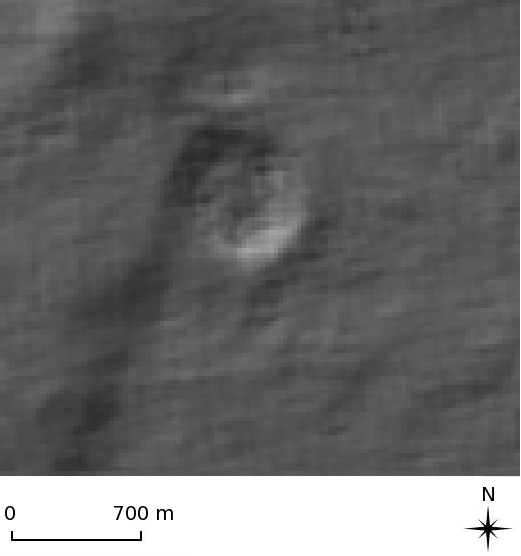
\includegraphics[width=0.4\textwidth]{hires_dem.jpg}
\caption[sfs]{The CTX DEM, gridded at 24 meters/pixel (hence 4x the image resolution), that is used to optimize the image exposure, haze, and reflectance model coefficients.}
\label{hires}
\end{figure}

\begin{figure}[h!]
\centering
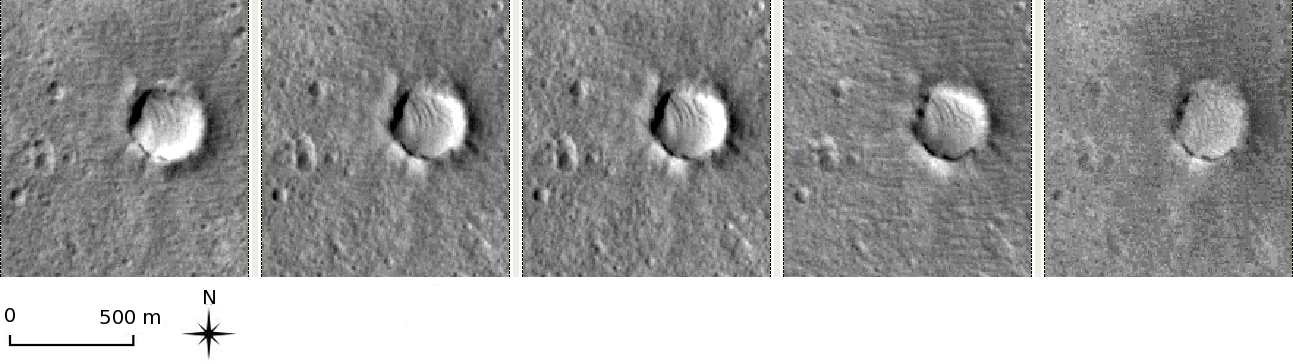
\includegraphics[width=\textwidth]{sfs_mars_fig1}
\caption[sfs]{The five CTX images used in this example, shown from left to right in the same order as from top to bottom in Table \ref{ctximages}.}
\label{sfs1}
\end{figure}

We started by bundle-adjusting all of the images using ASP to eliminate camera errors, then we used the second and the third images (which were acquired with similar illumination) to create a CTX DEM with ASP's \texttt{stereo} program. 

While the CTX images have a ground sample distance on the order of 6 meters/pixel, a terrain model obtained from them will have an effective resolution that will be coarser by a factor of 4 or even more. Hence, we created the terrain model at 24 meters/pixel, which shows a reasonable amount of detail. The DEM we used is shown in Figure \ref{hires}. 

As described in section \ref{twostep}, we used this terrain model to solve the SfS problem while keeping this terrain fixed, and varying only the image exposures, haze values, and reflectance model coefficients, which are resolution-independent. The images used here were also resampled, for consistency, to the same 4x coarser resolution using the USGS ISIS \texttt{reduce} tool.  

At the next step, we considered the same terrain model created with stereo as above, yet chose a clip from it that was not overlapping, but was close, to the one used earlier to determine the image and model parameters. This is meant to show that our SfS algorithm is able to generalize, to some extent, and it need not be used on precisely the same region it was trained on. We gridded this clip at 6 meters/pixel, and we employed the original CTX images to refine this terrain using SfS, while keeping fixed the image exposures, haze values, and reflectance model coefficients that we determined at the previous step.   

\begin{figure}[h!]
\centering
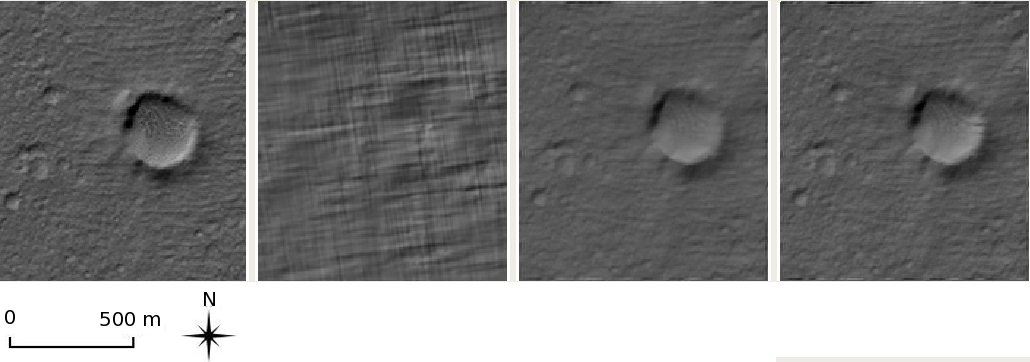
\includegraphics[width=0.8\textwidth]{sfs_mars_fig2}
\caption[sfs]{From left to right, the HiRISE DEM used for validation, the DEM obtained from CTX images at 6 meter/pixel, the refined SfS DEM obtained from the CTX images without modeling haze, and the refined SfS DEM while modeling haze.}
\label{sfs2}
\end{figure}

\begin{figure}[h!]
\centering
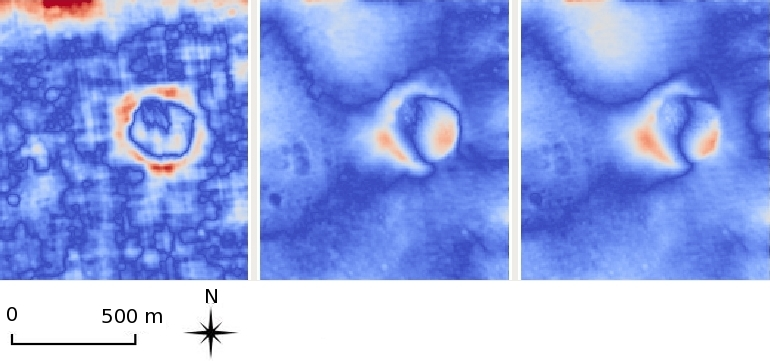
\includegraphics[width=0.6\textwidth]{sfs_mars_fig3}
\caption[sfs]{From left to right, the colorized absolute differences between the HiRISE DEM and each of: the initial guess to SfS, the SfS result without modeling haze, and the SfS result while modeling haze. The brightest shade of red corresponds to a 13 m error.}
\label{sfs3}
\end{figure}

We used the HiRISE terrain model DTEEC\_041937\_1920\_042003\_1920\_L01 at for validation. Its resolution is 1m/pixel, and we regridded it at 6 m/pixel to be consistent with the resolution we are working on. We aligned this terrain to the initial guess to SfS and computed the mean and standard deviation of the absolute difference of the two, which we call the errors \textit{before} SfS, and then we aligned this terrain to the DEM obtained via SfS and computed these measures again. We call those the errors \textit{after} SfS. 

Within this set up, we performed various experiments, by picking several of the images of the above for SfS, a reflectance model among the Lambertian, lunar-Lambertian, and Hapke, while varying or not their coefficients (this is not applicable to the Lambertian), and including or not the haze values as part of the problem. 

We present below two results. In the first, we used for SfS the first, second, fourth and fifth images in the table, while not modeling the atmospheric haze. We used the lunar-Lambertian model with optimized model coefficients. As result of SfS, the mean absolute difference to the aligned HiRISE model went from 2.40~m to 1.96~m, while its standard deviation decreased from 2.35~m to 1.56~m.

In the second experiment, we used the first, third, and fourth images while modeling the haze. We used, as before, the lunar-Lambertian model with optimized coefficients. The starting errors are the same as before. The mean absolute difference compared to the aligned HiRISE model decreased to 2.26~m while its standard deviation decreased to 1.70~m. 

In both of these examples we used $\mu=0.03$, $\nu=0.1$, and $\lambda=10^{-5}.$

We obtained very similar results if using instead the Hapke reflectance model while refining its coefficients just as for the lunar-Lambertian. We got worse results with the Lambertian model, or when not optimizing the coefficients of the models. 

In Figure \ref{sfs1} are shown the five images that are used in this example. In Figure \ref{sfs2} are presented the reference HiRISE DEM that is used for validation, the initial guess CTX DEM at 6 m/pixel, and two results from running SfS, one without modeling haze and second one while modeling it. The colorized absolute difference between the last three DEMs as compared to the reference HiRISE DEM is shown in Figure \ref{sfs3}. Lastly, a profile through some of the DEMs is shown in Figure \ref{profile}. 

It can be seen from these figures that SfS removes the numerical noise from the CTX DEM (the noise is expected, given that the effective resolution of the DEM is 4x the image resolution, and here it is created at 1x image resolution), adds a wealth of detail, and reconstructs correctly the crater rim. It can also be seen, based on the shades of red in Figure \ref{sfs3} that the accuracy of the obtained terrain models is worse where the images are very bright.   

\begin{figure}[h!]
\centering
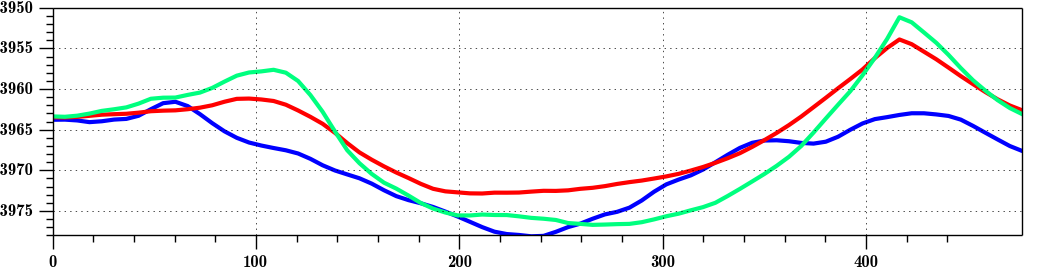
\includegraphics[width=0.8\textwidth]{profile.png}
\caption[sfs]{A profile of the DEMs in Figure \ref{sfs2} along a cutline going roughly vertically and through the middle of the crater. Profiled are the HiRISE DEM (green), initial guess to SfS (blue), and the SfS result when haze is not modeled (red).}
\label{profile}
\end{figure}


\section{Conclusions}

We showed that it is possible to use CTX images to refine terrain models on Mars, with and without modeling haze, and while tuning the reflectance model coefficients as part of the optimization. We validated our results with an independently created hi-resolution HiRISE DEM. 

The results look very promising. There is room for improvement in regions where the illumination produces the brightest spots. Either our modeling is not fully accurate there, or perhaps images are becoming saturated and the brightness values are not accurate. It will likely help to have images with more diverse illumination conditions, which may be a challenge with both CTX and HiRISE data, hence we would be inclined to also study other imagers in the future. We also plan to improve our modeling, and study how the images and reflectance model used impact the results. The ultimate goal is to use SfS with HiRISE images to refine the existing highest resolution terrains, which may help in landing future missions to Mars. 

%Text here ===>>>

%%

%  Numbered lines in equations:
%  To add line numbers to lines in equations,
%  \begin{linenomath*}
%  \begin{equation}
%  \end{equation}
%  \end{linenomath*}



%% Enter Figures and Tables near as possible to where they are first mentioned:
%
% DO NOT USE \psfrag or \subfigure commands.
%
% Figure captions go below the figure.
% Table titles go above tables;  other caption information
%  should be placed in last line of the table, using
% \multicolumn2l{$^a$ This is a table note.}
%
%----------------
% EXAMPLE FIGURE
%
% \begin{figure}[h]
% \centering
% when using pdflatex, use pdf file:
% \includegraphics[width=20pc]{figsamp.pdf}
%
% when using dvips, use .eps file:
% \includegraphics[width=20pc]{figsamp.eps}
%
% \caption{Short caption}
% \label{figone}
%  \end{figure}
%
% ---------------
% EXAMPLE TABLE
%
% \begin{table}
% \caption{Time of the Transition Between Phase 1 and Phase 2$^{a}$}
% \centering
% \begin{tabular}{l c}
% \hline
%  Run  & Time (min)  \\
% \hline
%   $l1$  & 260   \\
%   $l2$  & 300   \\
%   $l3$  & 340   \\
%   $h1$  & 270   \\
%   $h2$  & 250   \\
%   $h3$  & 380   \\
%   $r1$  & 370   \\
%   $r2$  & 390   \\
% \hline
% \multicolumn{2}{l}{$^{a}$Footnote text here.}
% \end{tabular}
% \end{table}

%% SIDEWAYS FIGURE and TABLE
% AGU prefers the use of {sidewaystable} over {landscapetable} as it causes fewer problems.
%
% \begin{sidewaysfigure}
% \includegraphics[width=20pc]{figsamp}
% \caption{caption here}
% \label{newfig}
% \end{sidewaysfigure}
%
%  \begin{sidewaystable}
%  \caption{Caption here}
% \label{tab:signif_gap_clos}
%  \begin{tabular}{ccc}
% one&two&three\\
% four&five&six
%  \end{tabular}
%  \end{sidewaystable}

%% If using numbered lines, please surround equations with \begin{linenomath*}...\end{linenomath*}
%\begin{linenomath*}
%\begin{equation}
%y|{f} \sim g(m, \sigma),
%\end{equation}
%\end{linenomath*}

%%% End of body of article

%%%%%%%%%%%%%%%%%%%%%%%%%%%%%%%%
%% Optional Appendix goes here
%
% The \appendix command resets counters and redefines section heads
%
% After typing \appendix
%
%\section{Here Is Appendix Title}
% will show
% A: Here Is Appendix Title
%
%\appendix
%\section{Here is a sample appendix}

%%%%%%%%%%%%%%%%%%%%%%%%%%%%%%%%%%%%%%%%%%%%%%%%%%%%%%%%%%%%%%%%
%
% Optional Glossary, Notation or Acronym section goes here:
%
%%%%%%%%%%%%%%
% Glossary is only allowed in Reviews of Geophysics
%  \begin{glossary}
%  \term{Term}
%   Term Definition here
%  \term{Term}
%   Term Definition here
%  \term{Term}
%   Term Definition here
%  \end{glossary}

%
%%%%%%%%%%%%%%
% Acronyms
%   \begin{acronyms}
%   \acro{Acronym}
%   Definition here
%   \acro{EMOS}
%   Ensemble model output statistics
%   \acro{ECMWF}
%   Centre for Medium-Range Weather Forecasts
%   \end{acronyms}
%
%%%%%%%%%%%%%%
% Notation
%   \begin{notation}
%   \notation{$a+b$} Notation Definition here
%   \notation{$e=mc^2$}
%   Equation in German-born physicist Albert Einstein's theory of special
%  relativity that showed that the increased relativistic mass ($m$) of a
%  body comes from the energy of motion of the body—that is, its kinetic
%  energy ($E$)—divided by the speed of light squared ($c^2$).
%   \end{notation}




%%%%%%%%%%%%%%%%%%%%%%%%%%%%%%%%%%%%%%%%%%%%%%%%%%%%%%%%%%%%%%%%
%
%  ACKNOWLEDGMENTS
%
% The acknowledgments must list:
%
% •	All funding sources related to this work from all authors
%
% •	Any real or perceived financial conflicts of interests for any
%	author
%
% •	Other affiliations for any author that may be perceived as
% 	having a conflict of interest with respect to the results of this
% 	paper.
%
% •	A statement that indicates to the reader where the data
% 	supporting the conclusions can be obtained (for example, in the
% 	references, tables, supporting information, and other databases).
%
% It is also the appropriate place to thank colleagues and other contributors.
% AGU does not normally allow dedications.


\acknowledgments

We gratefully acknowledge the Resource Prospector project at NASA Ames
Research Center for providing support for this research.

We would like to thank the anonymous reviewers for extremely thorough reviews and comments
of our paper \cite{alexandrovmulti} that we used in improving our software and our modeling for Mars. 


%% ------------------------------------------------------------------------ %%
%% Citations

% Please use ONLY \citet and \citep for reference citations.
% DO NOT use other cite commands (e.g., \cite, \citeyear, \nocite, \citealp, etc.).


%% Example \citet and \citep:
%  ...as shown by \citet{Boug10}, \citet{Buiz07}, \citet{Fra10},
%  \citet{Ghel00}, and \citet{Leit74}.

%  ...as shown by \citep{Boug10}, \citep{Buiz07}, \citep{Fra10},
%  \citep{Ghel00, Leit74}.

%  ...has been shown \citep [e.g.,][]{Boug10,Buiz07,Fra10}.



%%  REFERENCE LIST AND TEXT CITATIONS
%
% Either type in your references using
%
% \begin{thebibliography}{}
% \bibitem[{\textit{Kobayashi et~al.}}(2003)]{R2013} Kobayashi, T.,
% Tran, A.~H., Nishijo, H., Ono, T., and Matsumoto, G.  (2003).
% Contribution of hippocampal place cell activity to learning and
% formation of goal-directed navigation in rats. \textit{Neuroscience}
% 117, 1025--1035.
%
% \bibitem{}
% Text
% \end{thebibliography}
%
%%%%%%%%%%%%%%%%%%%%%%%%%%%%%%%%%%%%%%%%%%%%%%%
% Or, to use BibTeX:
%
% Follow these steps
%
% 1. Type in \bibliography{<name of your .bib file>}
%    Run LaTeX on your LaTeX file.
%
% 2. Run BiBTeX on your LaTeX file.
%
% 3. Open the new .bbl file containing the reference list and
%   copy all the contents into your LaTeX file here.
%
% 4. Run LaTeX on your new file which will produce the citations.
%
% AGU does not want a .bib or a .bbl file. Please copy in the contents of your .bbl file here.

\bibliography{sfs_mars}


%% After you run BibTeX, Copy in the contents of the .bbl file here:




%%%%%%%%%%%%%%%%%%%%%%%%%%%%%%%%%%%%%%%%%%%%%%%%%%%%%%%%%%%%%%%%%%%%%
% Track Changes:
% To add words, \added{<word added>}
% To delete words, \deleted{<word deleted>}
% To replace words, \replaced{<word to be replaced>}{<replacement word>}
% To explain why change was made: \explain{<explanation>} This will put
% a comment into the right margin.

%%%%%%%%%%%%%%%%%%%%%%%%%%%%%%%%%%%%%%%%%%%%%%%%%%%%%%%%%%%%%%%%%%%%%
% At the end of the document, use \listofchanges, which will list the
% changes and the page and line number where the change was made.

% When final version, \listofchanges will not produce anything,
% \added{<word or words>} word will be printed, \deleted{<word or words} will take away the word,
% \replaced{<delete this word>}{<replace with this word>} will print only the replacement word.
%  In the final version, \explain will not print anything.
%%%%%%%%%%%%%%%%%%%%%%%%%%%%%%%%%%%%%%%%%%%%%%%%%%%%%%%%%%%%%%%%%%%%%

%%%

\listofchanges

%%%

\end{document}

%%%%%%%%%%%%%%%%%%%%%%%%%%%%%%%%%%%%%
%% Supporting Information
%% (Optional) See AGUSuppInfoSamp.tex/pdf for requirements
%% for Supporting Information.
%%%%%%%%%%%%%%%%%%%%%%%%%%%%%%%%%%%%%



%%%%%%%%%%%%%%%%%%%%%%%%%%%%%%%%%%%%%%%%%%%%%%%%%%%%%%%%%%%%%%%

More Information and Advice:

%% ------------------------------------------------------------------------ %%
%
%  SECTION HEADS
%
%% ------------------------------------------------------------------------ %%

% Capitalize the first letter of each word (except for
% prepositions, conjunctions, and articles that are
% three or fewer letters).

% AGU follows standard outline style; therefore, there cannot be a section 1 without
% a section 2, or a section 2.3.1 without a section 2.3.2.
% Please make sure your section numbers are balanced.
% ---------------
% Level 1 head
%
% Use the \section{} command to identify level 1 heads;
% type the appropriate head wording between the curly
% brackets, as shown below.
%
%An example:
%\section{Level 1 Head: Introduction}
%
% ---------------
% Level 2 head
%
% Use the \subsection{} command to identify level 2 heads.
%An example:
%\subsection{Level 2 Head}
%
% ---------------
% Level 3 head
%
% Use the \subsubsection{} command to identify level 3 heads
%An example:
%\subsubsection{Level 3 Head}
%
%---------------
% Level 4 head
%
% Use the \subsubsubsection{} command to identify level 3 heads
% An example:
%\subsubsubsection{Level 4 Head} An example.
%
%% ------------------------------------------------------------------------ %%
%
%  IN-TEXT LISTS
%
%% ------------------------------------------------------------------------ %%
%
% Do not use bulleted lists; enumerated lists are okay.
% \begin{enumerate}
% \item
% \item
% \item
% \end{enumerate}
%
%% ------------------------------------------------------------------------ %%
%
%  EQUATIONS
%
%% ------------------------------------------------------------------------ %%

% Single-line equations are centered.
% Equation arrays will appear left-aligned.

Math coded inside display math mode \[ ...\]
 will not be numbered, e.g.,:
 \[ x^2=y^2 + z^2\]

 Math coded inside \begin{equation} and \end{equation} will
 be automatically numbered, e.g.,:
 \begin{equation}
 x^2=y^2 + z^2
 \end{equation}


% To create multiline equations, use the
% \begin{eqnarray} and \end{eqnarray} environment
% as demonstrated below.
\begin{eqnarray}
  x_{1} & = & (x - x_{0}) \cos \Theta \nonumber \\
        && + (y - y_{0}) \sin \Theta  \nonumber \\
  y_{1} & = & -(x - x_{0}) \sin \Theta \nonumber \\
        && + (y - y_{0}) \cos \Theta.
\end{eqnarray}

%If you don't want an equation number, use the star form:
%\begin{eqnarray*}...\end{eqnarray*}

% Break each line at a sign of operation
% (+, -, etc.) if possible, with the sign of operation
% on the new line.

% Indent second and subsequent lines to align with
% the first character following the equal sign on the
% first line.

% Use an \hspace{} command to insert horizontal space
% into your equation if necessary. Place an appropriate
% unit of measure between the curly braces, e.g.
% \hspace{1in}; you may have to experiment to achieve
% the correct amount of space.


%% ------------------------------------------------------------------------ %%
%
%  EQUATION NUMBERING: COUNTER
%
%% ------------------------------------------------------------------------ %%

% You may change equation numbering by resetting
% the equation counter or by explicitly numbering
% an equation.

% To explicitly number an equation, type \eqnum{}
% (with the desired number between the brackets)
% after the \begin{equation} or \begin{eqnarray}
% command.  The \eqnum{} command will affect only
% the equation it appears with; LaTeX will number
% any equations appearing later in the manuscript
% according to the equation counter.
%

% If you have a multiline equation that needs only
% one equation number, use a \nonumber command in
% front of the double backslashes (\\) as shown in
% the multiline equation above.

% If you are using line numbers, remember to surround
% equations with \begin{linenomath*}...\end{linenomath*}

%  To add line numbers to lines in equations:
%  \begin{linenomath*}
%  \begin{equation}
%  \end{equation}
%  \end{linenomath*}

